Þegar taka þarf röð ákvarðana  yfir tímabil geta ákvarðanir sem teknar eru snemma í ferlinu haft áhrif á gæði þeirra sem síðar eru teknar. Ef skammtíma sjónarmið ráða eingöngu för, fæst niðurstaða sem yfirleitt er frábrugðin bestu mögulegu lausn. \ath{Kvika bestun} má oft nota bestu röð aðgerða.

\begin{description}
\item[\ath{Þrep}] (e. stages): hvert verkefni hefur $N$ þrep (tímaþrep) táknað með $n$ og á hverju þrepi er tekin ákvörðun $x_n$.
\item[\ath{Staða}] (e. state): á hverju þrepi $n$ eru nokkrar stöður $s_n$.
\item[\ath{Ákvörðun}] (e. action or policy decision): er byggð á $f_{n}^*(s_{n})$ þar sem $x^*_n$ er besta ákvörðunin á þrepi $n$ (lágmarka eða hámarka):
  $$f_n^*(s_n) = f_n(s_n,x_n^*) = \min_{x_n} f_n(s_n,x_n) \mbox{ eða } \max_{x_n} f_n(s_n,x_n)$$
\item[\ath{Besta stefna}] (e. optimal policy): markmið aðferðarinnar er að finna stefnu $\pi$ sem segir til um hvaða ákvörðun sé best $x^*_n = \pi^*(s_n)$ í hverju þrepi.
\item[\emph{$f_n(s_n,x_n)$}]  Tillegg til markfalls á þrepum $n,\ldots, N$ ef tekin er ákvörðun $x_n$ og síðan bestu ákvarðanir eftir það (á þrepum $n+1, \ldots, N$).
\item[\ath{Kostnaður}] $\mathcal{C}_{s_ns_{n+1}}^{x_n}$ er kostnaður við að taka ákvörðun $x_n$ og fara úr stöðu $s_n$ í stöðu $s_{n+1}$.
\item[\ath{Slembin kvik bestun}] (e. stochastic): $\mathcal{P}_{s_ns_{n+1}}^{x_n}$ er líkur á að fara úr stöðu $s_n$ í stöðu $s_{n+1}$ þegar ákvörðun $x_n$ er tekin. Í þessu   tilfelli er $f_n$ væntigildi (meðaltal).
\item[\ath{Óslembin kvik bestun}] (e. deterministic):
$$f_n^*(s_n) = \min_{x_n} \Big(\mathcal{C}_{s_ns_{n+1}}^{x_n}+ \alpha f_{n+1}^*(s_{n+1})\Big)$$
\item[\ath{Markov-eiginleiki}] gefið að við séum í stöðu $s_n$, þá er besta ákvörðun fyrir þau ástönd sem á eftir koma óháð því hvaða ákvarðanir voru teknar á fyrri þrepum   ($x_{n-1}, x_{n-2}, \ldots$).
\item[\ath{$N=\infty$}] þá stefnir $f_n\rightarrow\infty$, og því þarf $0 < \alpha <1$ (e. discount factor), annars notum við venjulega $\alpha=1$ þegar $N$ er takmarkað.
\item[\ath{Bellman-jafna}]
$$f_n^*(s_n) = \min_{x_n} \sum_{s_{n+1}\in
  s'}\mathcal{P}_{s_ns_{n+1}}^{x_n}\Big(\mathcal{C}_{s_ns_{n+1}}^{x_n}+ \alpha f_{n+1}^*(s_{n+1})\Big)$$
\end{description}
\begin{center}
\begin{figure}[h!]
  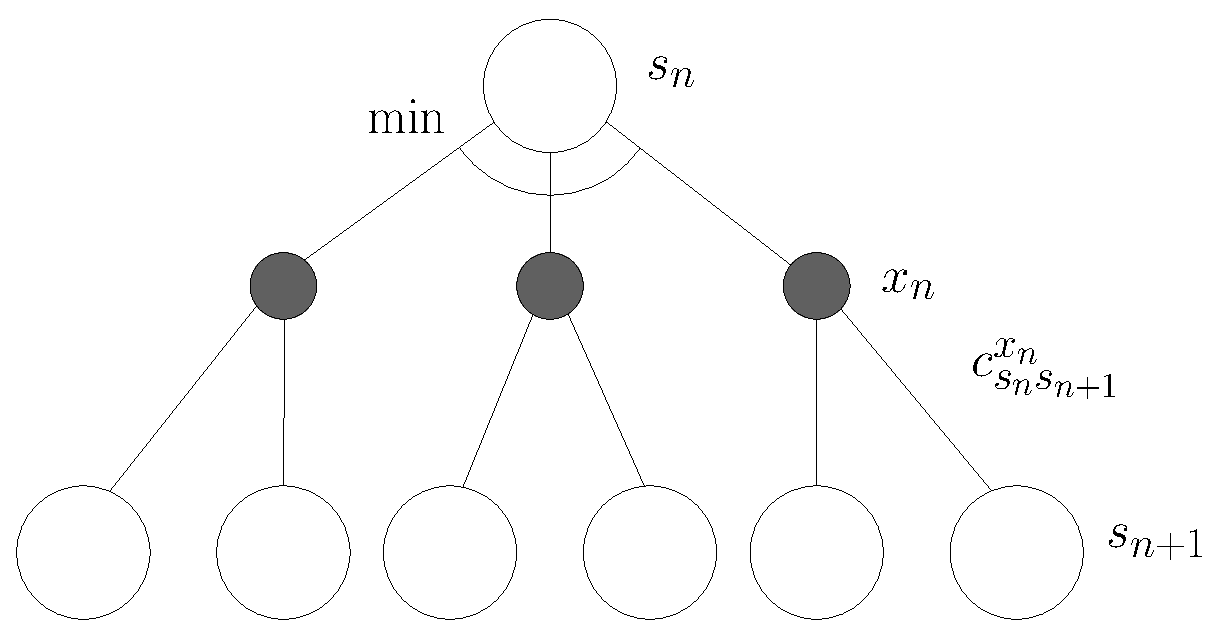
\includegraphics[width=0.9\columnwidth]{figs/stateaction.eps}
\end{figure}
\end{center}

\section{Aðferðin}
\begin{itemize}
\item Aðferð virkar með því að vinna sig afturábak frá  $n=N,N-1,\ldots,2,1$. 
\item Lesum bestu lausn áfram frá $n=1$.
\item Gefin besta ákvörðun í þrepi $n+1$ þá finnum við bestu ákvörðun í þrepi $n$ með því að nota \ath{endurkvæma sambandið} (e. recursive relationship), sem dæmi: 
$$f_n^*(s_n) = \min_{x_n} \Big(\mathcal{C}_{s_ns_{n+1}}^{x_n}+ f_{n+1}^*(s_{n+1})\Big)$$
\end{itemize}
\newpage
\begin{samepage}
\begin{aths}Afturvirka sambandið þarf ekki að vera línulegt,  annað dæmi um afturvirkt samband er 
$$f_n^*(s_n) = \min_{x_n} \Big(\mathcal{C}_{s_ns_{n+1}}^{x_n} f_{n+1}^*(s_{n+1})\Big)$$
 \end{aths}
\end{samepage}


Í kvikri bestun er oft \emph{unnið afturábak}. Oft er engan veginn augljóst hvernig leysa á bestunarverkefni með kvikri bestun -- listgrein frekar en vísindi. Best er að læra það m.þ.a. skoða (og leysa) nokkur dæmi.


\begin{daemi}[Leikur] Höfum eftirfarandi leikreglur:
  \begin{itemize}
    \item Tveir leikmenn
    \item 30 eldspýtur
    \item Leikmenn skiptast á að draga 1, 2 eða 3 eldspýtur
    \item Sá sem á leik þegar ein eldspýta er eftir tapar
  \end{itemize}
Hvernig getur sá sem byrjar tryggt sér sigur?
\end{daemi}
\begin{lausn}Setjum möguleg ástönd og aðgerðir upp í töflu.
\begin{center}
  \begin{tabular}{|cc|} \hline
    Fjöldi sem er eftir & Fjöldi eldspýta sem degnar eru \\
    (ástand) 		& (aðgerð) \\ \hline 
    \fbox{1}		&  tapar	\\ 
    2			&  1	\\ 
    3			&  2	\\ 
    4			&  3	\\ 
    \fbox{5}		&  tapar	\\ 
    6			&  1	\\ 
    7			&  2	\\ 
    8			&  3	\\  
    \fbox{9}		& tapar	\\ 
    $\vdots$		& \vdots	\\ \hline 
\end{tabular}
\end{center}
Ástönd sem leiða t.þ.a. andstæðingur tapar eru $T=\{1,5,9,13,17,21,25,29\}$.

Drögum eina eldspýtu í upphafi. Í framhaldinu er fjöldinn valinn þannig að andstæðingur lendi í einu af ástöndum $T$.
\end{lausn}

\begin{daemi}[Afbrigði af svonefndu \emph{bakpokaverkefni}]%\footnote{Sjá \href{http://en.wikipedia.org/wiki/Knapsack\_problem}{Knapsack problem}}]
Vörubíll getur í mesta lagi borið 10 tonna farm. Hægt er að senda þrjár mismunandi vörur með bílnum $V1,V2$ og $V3$. Þyngd og verðmæti eru:
\[ \begin{array}{|cl|ccc|} \hline
     & & V1 & V2 & V3 \\ \hline
    w & \mbox{þyngd (tonn)} & 1 & 2 & 2 \\
    u & \mbox{verðmæti} & 200 & 500 & 600 \\ \hline
   \end{array}\]
A.m.k. eitt stykki af hverri vöru á að fara í bílinn. 
Hvernig á að ferma bílinn þ.a. heildarverðmæti sé hámarkað?
\end{daemi}

\begin{lausn}\hspace{.1cm}

\begin{center}
\begin{tabular}{ll}
    Þrep & vara $i=1,2,3$. \\
    Ástand & $s_n=$ rými sem eftir er að ráðstafa á þrepi $n$\\
    Ákv.br.&  $x_n=$ magn sem sent er af vöru $i$ á þrepi $n$
\end{tabular}
\end{center}
\begin{aths}Þurfum að taka a.m.k. eitt stk. af hverri vöru $\Rightarrow$ 3 \emph{þrep} í verkefninu. Athugið einnig að þrepið er ekki tími, eins og oft er raunin í kvikri bestun).\end{aths}

Virði þess að taka ákvörðun $x_n$ á þrepi $n$ (og taka alltaf bestu ákvörðun eftir það) er gefið með eftirfarandi jöfnu:
$$ f_n(s_n)=x_n\cdot\underbrace{u_n}_{\tiny \mbox{verðmæti/ein}}+f^k_{n+1}(s_n-x_n\cdot\underbrace{w_n}_{\tiny \mbox{þyngd/ein}})$$

\begin{description}
  \item[Þrep $n=3$] Hér er um að ræða vöru 3, $w_3=2$ og $u_3=600$: Á þessu þrepi erum við búin að setja vörur 1 og 2 í bílinn og því mest $10-1-2=7$ tonn laus.
  \[\begin{array}{|c|c|c|}\hline 
    s_3 & f_3^*(s_3) & x_3^* \\ \hline 
    7	& 3\cdot600 & 3 \\
    6	& 3\cdot600 & 3 \\
    5	& 2\cdot600 & 2 \\
    4	& 2\cdot600 & 2 \\
    3	& 1\cdot600 & 1 \\
    2	& 1\cdot600 & 1 \\    \hline
    \end{array}\]
  \item[Þrep $n=2$] Hér er um að ræða vöru 2, $w_2=2$ og $u_2=500$: Á þessu þrepi erum við búin að setja vöru 1 í bílinn og því mest $10-1=9$ tonn laus.
  \[\begin{array}{|c|ccc|c|c|}\hline 
    s_2\backslash x_2 & \multicolumn{3}{c|}{f_2(s_2,x_2)=x_2u_2+f^*_3(s_2-x_2w_2)} &f_2^*(s_2)&  x_2^* \\ 
	& x_2=1	&	x_2=2	&	x_2=3	&	&	\\\hline 
    9	& 1\cdot500+1800 	& 2\cdot500+1200 	& 3\cdot600 	&2300	&	1\\
    8	& 1\cdot500+1800 	& 2\cdot500+1200 	& 3\cdot600 	&2300	&	1\\    
    7	& 1\cdot500+1200 	& 2\cdot500+600 	& - 		&1700	&	1\\
    6	& 1\cdot500+1200 	& 2\cdot500+600 	& -		&1700	&	1\\
    5	& 1\cdot500+600 	& - 			& - 		&1100	&	1\\
    4	& 1\cdot500+600 	& -			& - 		&1100	&	1\\
    \hline
    \end{array}\]
  \item[Þrep $n=1$] Hér er um að ræða vöru 1, $w_1=1$ og $u_1=200$: Á þessu þrepi er bílinn tómur og því 10 tonn til umráðanna
  \[\begin{array}{|c|cccccc|c|c|}\hline 
    s_1\backslash x_1 & \multicolumn{6}{c|}{f_1(s_1,x_1)=x_1u_1+f^*_2(s_1-x_1w_1)} &f_1^*(s_1)&  x_1^* \\ 
	& 1 & 2 & 3&4&5&6&&	\\\hline 
    10	& 1\cdot200	&2\cdot200	&3\cdot200&4\cdot200&5\cdot200&6\cdot200& 2700	&	2\\
    	& +2300 	&+2300		&+1700&+1700&+1100&+1100& &	\\
    \hline
    \end{array}\]
\end{description}
Sjáum strax hvað besta gildi markfalls er, nefnilega $z^*=f_1^*(s_1)=2700$. Til að finna bestu lausnina, þá þurfum við að lesa hana afturábak: $$x_1^*=2 \stackrel{s_2=8}{\longrightarrow} x_2^*=1\stackrel{s_3=6}{\longrightarrow} x_3^*=3.$$
\end{lausn}

\begin{comment}
Í kvikri bestun eru teknar ákvarðanir (e. decision) á \ath{þrepum} (e. stage) verkefnisins. Á sérhverju þrepi koma eitt eða fleiri \ath{ástönd} (e. stage) til greina. Ákvörðun í einhverju ástandi á tilteknu ástandi leiðir til \ath{færslu} (e. transition) yfir í ástand á næsta þrepi.

Svarandi til sérhvers (þrep,ástand) er \ath{virðisfall} (e. value function) sem er besta gildi á markfalli sem hægt er að ná m.þ.a. byrja í viðkomandi ástandi (og hegða sér optimalt eftir það).

\ath{Endurkvæmt samband} (e. recursive relation) ríkir milli virðisfalla fyrir mismunandi ástönd.

Safn ákvarðana fyrir öll  mögulega ástönd mynda \ath{stefnureglu} (e. policy) ákvarðanatakans. Erum að leita að bestu stefnureglu í tilteknu verkefni. 

Látum 
\begin{enumerate}
  \item[$N$] fjöldi þrepa
  \item[$n$] núverandi þrep ($n\in\{1,..,N\}$
  \item[$s_n$] ástand á þrepi $n$
  \item[$x_n$] ákvörðun á þrepi $n$
  \item[$x_n^*$] besta gildi $x_n$ (gefið $s_n$)
  \item[$f_n(s_n,x_n)$] framlag þrepa $n,n+1,..,N$ til markfallsins m.v. að byrjað sé í ástandi $s_n$ á þrepi $n$, ákvörðun $x_n$ sé þekkt og bestu ákvarðanir séu teknar þar á eftir.
  \item[$f_n^*(s_n,x_n)$] $=\max_{x_n} f_n(s_n,x_n)$ (eða $\min$)
\end{enumerate}

\begin{center}
  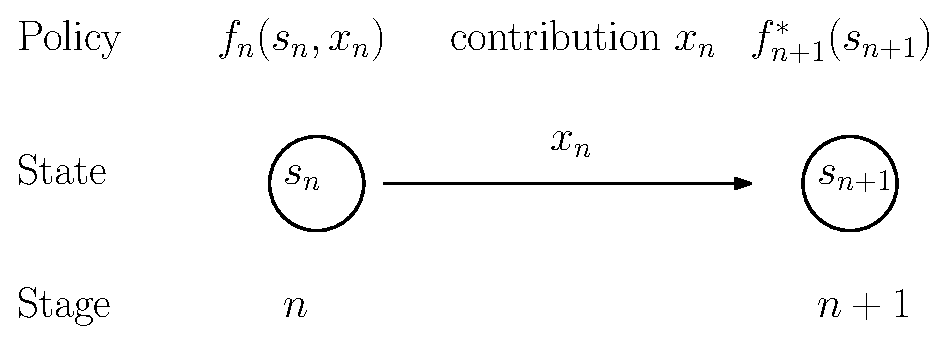
\includegraphics[width=0.5\columnwidth]{figs/stagestep.eps}
\end{center}
\end{comment}

\begin{daemi}[Skipan rannsóknateyma]Höfum gefnar forsendur:
  \begin{itemize}
    \item Þrjú teymi glíma við sama verkefnið (geimferðaáætlun) en nota mismunandi aðferðir
    \item Líkur á að hópunum \emph{mistakist} að leysa verkefnið hefur verið metnar eftirfarandi:
    \[\begin{matrix}       1 & 0.4 \\ 2 & 0.6 \\ 3 & 0.8       \end{matrix}\]
    Líkur að öllum mistekist er því $0.4\cdot0.6\cdot0.8=0.192$.
  \end{itemize}
  Nú bætast við tveir toppmenn við í verkefnið. Hvernig á að ráðstafa þessum nýju mönnum þ.a. líkur á að öllum hópum mistakist séu lágmarkaðar m.v. að líkur á að mistakast séu eftirfarandi:
 \[\begin{array}{|c|ccc|} \hline \mbox{fj. sem } & \multicolumn{3}{c|}{\mbox{Hópur}}\\
  \mbox{bætist við}& 1 & 2 & 3 \\ \hline
  0 & 0.4 & 0.6 & 0.8 \\
  1 & 0.2 & 0.4 & 0.5 \\
  2 & 0.15 & 0.2 & 0.3    \\\hline   
   \end{array}\]
\end{daemi}
\begin{lausn}Látum
%Er raunhæft að finna bestu lausn m.þ.a. prófa einfaldlega alla möguleika?  
\begin{center}\begin{tabular}{lp{7cm}}
  Þrep $n$ & teymi $1,2,3$ \\
  Ástand $s_n$ &  fjöldi sem \emph{eftir} er að ráðstafa á þrepin \\
  Ákv.br. $x_n$ & fjöldi sem úthlutað er á hóp $n$ \\
  $p_i(x_i)$ & líkur á að teymi $i$ mistakist m.v. að $x_i$ mönnum hafi verið bætt við hóp $i$.
\end{tabular}\end{center}
Líkur á að öllum mistakist eru $p(x_1)p(x_2)p(x_3)$. Lágmörkum þá stærð, þ.e.
  $$ \min_{\vec{x}} p(x_1)p(x_2)p(x_3)$$
m.t.t. sk. $$x_1+x_2+x_3=2$$ $$x_i\geq0,~~x_i\mbox{ heiltölur}$$
Þá er 
$$f_n(s_n,x_n)=p_n(x_n)f^*_{n+1}(s_n-x_n)$$
með
$$f_n^*(s_n,x_n)=\min_{x_n\in\{0,..,s_n\}}f_n(s_n,x_n)$$
  
\begin{description}
  \item[Þrep $n=3$]
{\scriptsize
  \[\begin{array}{|c|c|c|}\hline 
    s_3 & f_3^*(s_3) & x_3^* \\ \hline 
    0	& 0.8 & 0 \\
    1	& 0.5 & 1 \\
    2	& 0.3 & 2 \\    \hline
    \end{array}\]}
  \item[Þrep $n=2$]
{\scriptsize
  \[\begin{array}{|c|ccc|c|c|}\hline 
    s_2\backslash x_2 & \multicolumn{3}{c|}{f_2(s_2,x_2)=p_2(x_2)f^*_3(s_2-x_2)} &f_2^*(s_2)&  x_2^* \\ 
	& x_2=0	&	x_2=1	&	x_2=2	&	&	\\\hline 
    0	& 0.6\cdot0.8=0.48 	& - 	& - & 0.48&	0\\
    1	& 0.6\cdot0.5=0.30 	& 0.4\cdot0.8=0.32 	& - &0.3&	0\\    
    2	& 0.6\cdot0.3=0.18 	& 0.4\cdot0.5=0.2 	& 0.2\cdot0.8=0.16	&0.16&	2\\
    \hline
    \end{array}\]}
  \item[Þrep $n=1$]
{\scriptsize 
  \[\begin{array}{|c|ccc|c|c|}\hline 
    s_1\backslash x_1 & \multicolumn{3}{c|}{f_1(s_1,x_1)=p_1(x_1)f^*_2(s_1-x_1)} &f_1^*(s_1)&  x_1^* \\ 
	& x_1=0	&	x_1=1	&	x_1=2	&	&	\\\hline 
    2	& 0.4\cdot0.16=0.064 	& 0.2\cdot0.3=0.06 	& 0.15\cdot0.48=0.072	&0.06&	1\\
    \hline
    \end{array}\]}
\end{description}
Besta lausn er $$x_1^*=1\stackrel{s_2=1}{\longrightarrow}x_2^*=0\stackrel{s_3=1}{\longrightarrow}x_3^*=1$$ sem gefur líkurnar að öllum mistekist eru 0.06.

\end{lausn}
\begin{daemi}[Lagerhald]
  Fyrirtæki framleiðir eina tegund vöru og selur áfram.
  \begin{center}\begin{tabular}{ll}
    $d_j$ & Eftirspurn í mánuði $j$ (gefin) \\
    $x_j$ & Magn sem á að framleiða (ákv.breyta) \\
    $i_j$ & Lagerstaða í upphafi $j$-ta tímabils (ástand)
  \end{tabular}\end{center}
Í mánuði $i$ gildir
$$i_{j+1}=i_j+x_j-d_j$$
G.r.f. að $i_1$ sé þekkt (upphafsstaða) og lager verði tómur í lokin. Að auki er g.r.f. að $d_j,i_j$ og $x_j$ séu heiltölur.

Kostnaður vegna framleiðslu í mánuði $j$ er
$$ \mathcal{C}_j(x_j)=\Bigg\{\begin{array}{cl} 0 & \mbox{ef } x_j=0\\ K_j+c_j(x_j) & \mbox{ef } x_j\geq0\end{array}$$
þar sem $K_j$ er uppsetningarkostnaður í mánuði $j$ og $c_j$ er einhver kostnaður háður  magni.

Þessu til viðbótar er birgðahaldskostnaður $h_j$ á einingu í mán. $j$. 
Hver eru þrep, ástönd, ákvarðanabreytur og virðisfall verkefnisins?
\end{daemi}
\begin{lausn}\hspace{.1cm}

\begin{center}  \begin{tabular}{lp{10cm}}
    Þrep &  tímabil $n\in\{1,2,..,N\}$ \\
    Ástand & lagerstaða í lok tímabils $j$, þ.e. $i_{j+1}$ \\
    Ákv.br. & $x_j$ er hversu mikið á að framleiða í mán. $j$ \\
    Virðisfallið & er heildarkostnaður: $ f(x_j,i_{j+1})=\mathcal{C}_j(x_j)+h_ji_{j+1}.$
  \end{tabular}\end{center}
\end{lausn}

\begin{daemi}[Birgðastýring]
  \[\begin{array}{|cccc|}\hline
    \mbox{Tímabil} & \mbox{Eftirspurn} (d_j) & \mbox{Upps.kostn} (K_j) & \mbox{Lagerk.} (h_j) \\\hline
1 & 3 & 3 & 1 \\
2 & 2 & 7 & 3 \\
3 & 4 & 6 & 2 \\ \hline
  \end{array}\]
Breytilegur kostnaður er $c_j=10$ fyrir fyrstu 3 einingarnar og 20 fyrir þær sem eru umfram það. Í upphafi er $i_1=1$.
\end{daemi}
\newpage
\begin{lausnSYND}\hspace{.1cm}
\begin{description}
  \item[Þrep $n=1$] Hér er $d_1=3$ en við höfum $i_1=1$, því framleiðum við minnst $x_1=d_1-i_1=2$ og til að dekka alla mögulegar framtíðar eftirspurnir þá þarf $x_1\leq d_2+d_3=2+4$. Því skoðum við $x_1\in\{2,..,6\}$.

Þurfum á $\mathcal{C}_1(x_1)$ að halda í töflunni:
\[ \begin{array}{cccccccc} x_1 & 2 &3&4&5&6&7&8\\\hline\mathcal{C}_1(x_1)&23&33&53&73&93&113&133\end{array}\]
{\scriptsize
\[\begin{array}{|cc|ccccccc|c|c|}\hline
  i_2 & h_1i_2 & \multicolumn{7}{c|}{f_1^*(i_2)=\mathcal{C}_1(x_1)+h_1i_2} & f^*(i_2) & x_1^* \\
\mbox{ástand} & \mbox{kostn} & 2 & 3 & 4 & 5 & 6 & 7 &8 &&\\ \hline 
0 & 0 & 23 &&&&&&& 23 & 2 \\
1 & 1 && 34 &&&&&& 34 & 3 \\
2 & 2 &&& 55 &&&&& 55 & 4 \\
3 & 3 &&&& 76 &&&& 76 & 5 \\
4 & 4 &&&&& 97 &&& 97 & 6 \\
5 & 5 &&&&&&118 && 118& 7 \\
6 & 6 &&&&&&& 139 & 139& 8 \\
\hline \end{array}\]}
\item[Þrep $n=2$]
\[ \begin{array}{cccccccc} x_2 & 0&1&2 &3&4&5&6\\\hline\mathcal{C}_2(x_2)&0&17&27&37&57&77&97\end{array}\]
{\scriptsize
\[\begin{array}{|cc|ccccccc|c|c|}\hline
  i_3 & h_2i_3 & \multicolumn{7}{c|}{f_2^*(i_3)=\mathcal{C}_2(x_2)+h_2i_3+f_1^*(i_3+d_2-x_2)} & f^*(i_3) & x_2^* \\
 &  & 2 & 3 & 4 & 5 & 6 & 7 &8 &&\\ \hline 
0 & 0 & 0+55 &17+34&27+23&-&-&-&-& 50 & 2 \\
1 & 3 &3+76& 20+55 &30+34&40+23&-&-&-& 63 & 3 \\
2 & 6 &6+97&23+76&33+55 &43+34&63+23&-&-& 77 & 3 \\
3 & 9 &9+118&26+97&36+76&46+55&66+34&86+23&-& 100 & 4 \\
4 & 12 &12+139&29+118&39+97&49+76&69+55&89+34&109+23& 123 & 5 \\
\hline \end{array}\]}
\item[Þrep $n=3$]
\[ \begin{array}{cccccc} x_3 & 0&1&2 &3&4\\\hline\mathcal{C}_3(x_3)&0&16&26&36&56\end{array}\]
{\scriptsize
\[\begin{array}{|cc|ccccc|c|c|}\hline
  i_4 & h_3i_4 & \multicolumn{5}{c|}{f_3^*(i_4)=\mathcal{C}_3(x_3)+h_3i_4+f_2^*(i_4+d_3-x_3)} & f^*(i_4) & x_3^* \\
 &  &0&1& 2 & 3 & 4 & &\\ \hline 
0 & 0 & 0+123&16+100&26+77&36+63&56+50&99&3\\
\hline \end{array}\]}
\end{description}
Besta lausn fæst m.þ.a. rekja sig afturábak:
$$\stackrel{i_4=0}{\longrightarrow}\fbox{$x_3^*=3$}\stackrel{i_3=i_4+d_3-x_3=1}{\longrightarrow}\fbox{$x_2^*=1$}\stackrel{i_2=i_3+d_2-x_2=0}{\longrightarrow}\fbox{$x_1^*=2$}$$ með heildarkostnað $z^*=99$.
\end{lausnSYND}


\section*{Mismunandi snið}
\[
\begin{array}{ll}
  \mathcal{C}_{s_n}(x_n)+f^*_{n+1}(s_{n+1}) & \min \sum_{n=1}^N \mathcal{C}_{s_n}(x_n) \\
  p_n(x_n)+f^*_{n+1}(s_n-x_n) & \max \sum_{n=1}^N p_n(x_n) \\
  p_n(x_n)\cdot f^*_{n+1}(s_n-x_n) & \max \prod_{n=1}^N p_n(x_n) \\
  x_nu_n+f^*_{n+1}(s_n-x_nw_n) & \max \sum_{n=1}^N x_nu_n \\
\end{array}
\]



\begin{comment}
\begin{daemi}[Spilavíti]
\begin{itemize}
\item Spilum $3$ leiki, $n=1,2,3$ (þrep).
\item Veðjum $x_n$ spilapeninga (ákvörðun).
\item Fjöldi spilapeninga er $s_n$ (staða).
\item Viljum hámarka líkur á að vera með $5$ peninga í lokin  (markmið).
\item Hvernig á að veðja? (besta stefna).
\item Gefið: P( vinnum $x$) $= \frac{2}{3}$, P( töpum $x$) $=\frac{1}{3}$.
\end{itemize}
Bellman jafna:
$$f_n^*(s_n) = \max_{x_n} \sum_{s_{n+1}\in
  s'}\mathcal{P}_{s_ns_{n+1}}^{x_n}\Big(\mathcal{C}_{s_ns_{n+1}}^{x_n}+ \alpha f_{n+1}^*(s_{n+1})\Big)$$
\end{daemi}
\begin{lausn}
 \begin{eqnarray*}
f_n(s_n) &=& \sum_{s_{n+1}\in  s'}\mathcal{P}_{s_ns_{n+1}}^{x_n} f_{n+1}^*(s_{n+1})\\
& =& \frac{1}{3}f_{n+1}^*(s_n-x_n)+\frac{2}{3}f_{n+1}^*(s_n+x_n)
\end{eqnarray*}
þar sem $f_4^*(s_4) = 0$ (terminal state) ef $s_4<5$ og $1$ ef $s_4\ge 5$.
Ritháttur: 
\begin{eqnarray*}
 x_n \textrm{ tapar}: & s_{n+1}=s_n-x_n \\
 x_n \textrm{ vinnur}: & s_{n+1}=s_n+x_n
\end{eqnarray*}
\vspace{5cm}
\begin{center}
  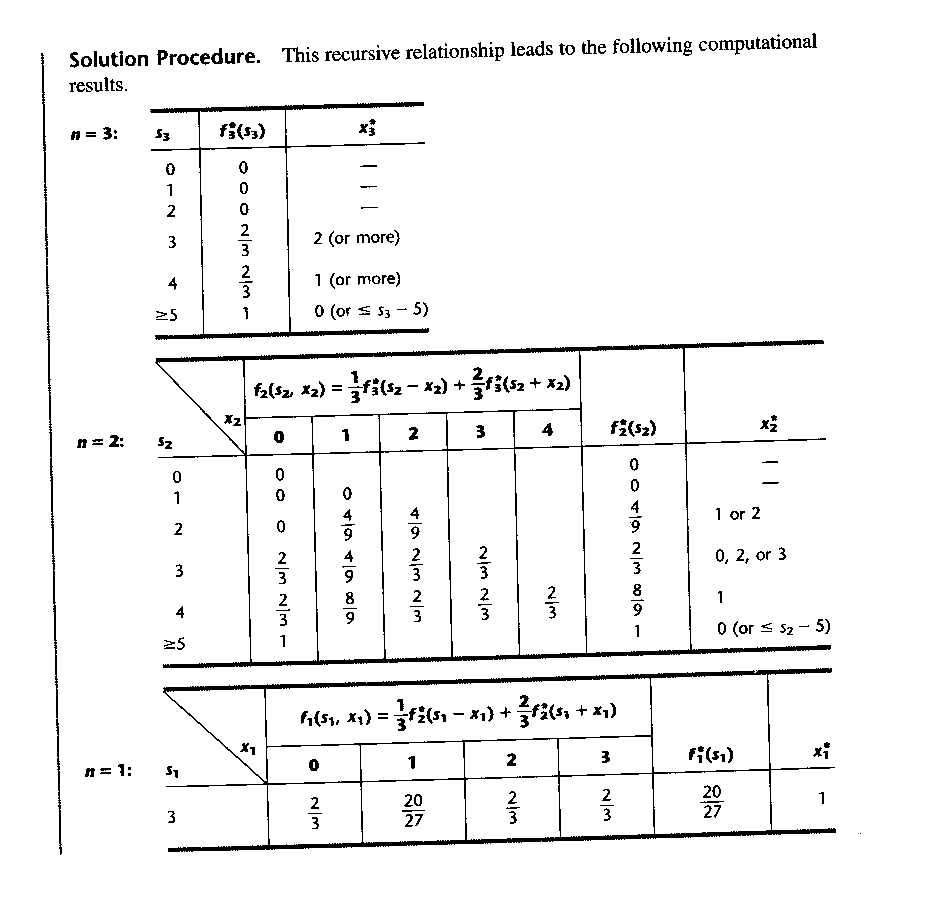
\includegraphics[width=0.9\columnwidth]{figs/spilaviti1.eps}
  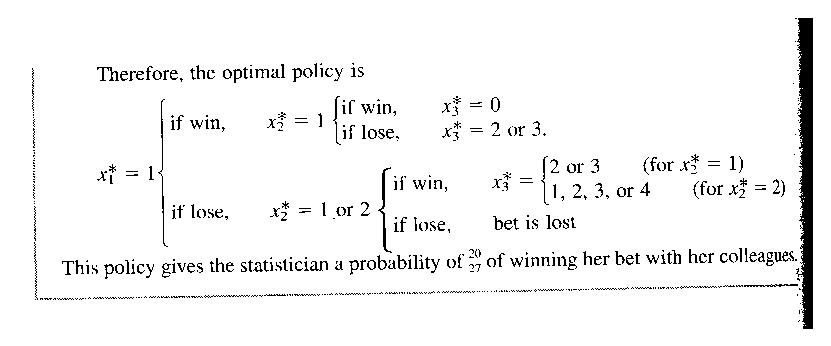
\includegraphics[width=0.9\columnwidth]{figs/spilaviti2.eps}
\end{center}
\end{lausn}


\begin{daemi}[Úthlutun á heilsugæsluteymum til vanþróaðra landa]Höfum fimm teymi sem úthluta þarf til þriggja landa. 

Hvernig á að úthluta teymunum til að hámarka jákvæð áhrif teymanna á heilsu landsmanna?

Aukning í fjölda mannára ef teymum er úthlutað á viðkomandi land:

\centering
\begin{tabular}{l|l|l|l}
\hline
Fjöldi teyma & land 1 & land 2 & land 3\\
\hline
0 & 0 & 0 & 0 \\
1 & 45 & 20 & 50 \\
2 & 70 & 45 & 70 \\
3 & 90 & 75 & 80 \\
4 & 105 & 110 & 100 \\
5 & 120 & 150 & 130 \\
\hline
\end{tabular}
\begin{center}
  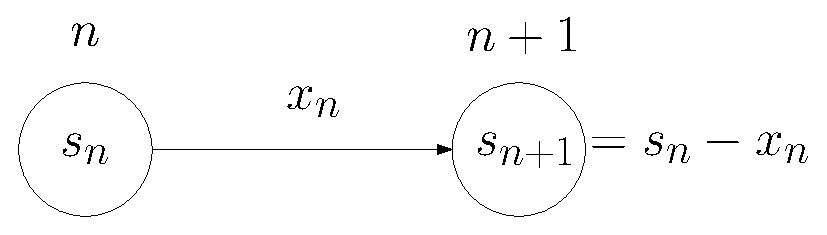
\includegraphics[width=0.5\columnwidth]{figs/teymi.eps}
\end{center}

\end{daemi}
\begin{lausn}
\begin{itemize}
\item {\bf Staða}: magn aðfanga til ráðstöfunar
\item $x_n$: magn aðfanga sem úthlutað er á þrepi $n$.
\end{itemize}Viljum leysa
$$\max_{x_1,x_2,x_3} ~~~ \sum_{i=1}^3 \mbox{jákvæð áhrif}
(x_i)$$
m.t.t. sk $$\sum_{i=1}^3 x_i = 5, \quad x_i \textrm{ eru jákvæðar heiltölur}.$$
\begin{center}
  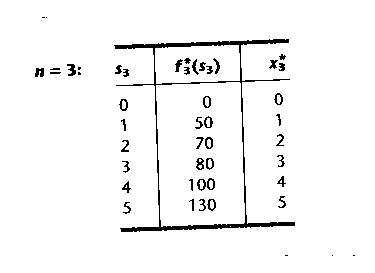
\includegraphics[width=0.5\columnwidth,angle=-2]{figs/teymi1.eps}
  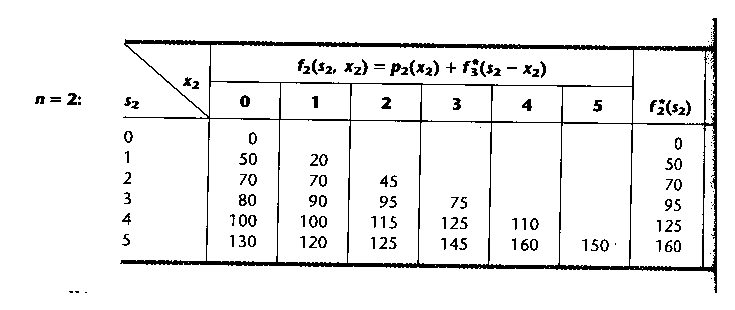
\includegraphics[width=0.9\columnwidth,angle=1]{figs/teymi2.eps}
  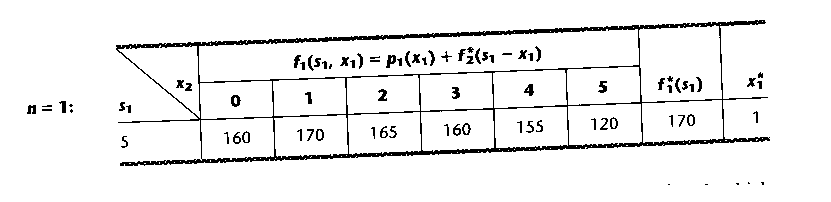
\includegraphics[width=0.9\columnwidth,angle=-2]{figs/teymi3.eps}
  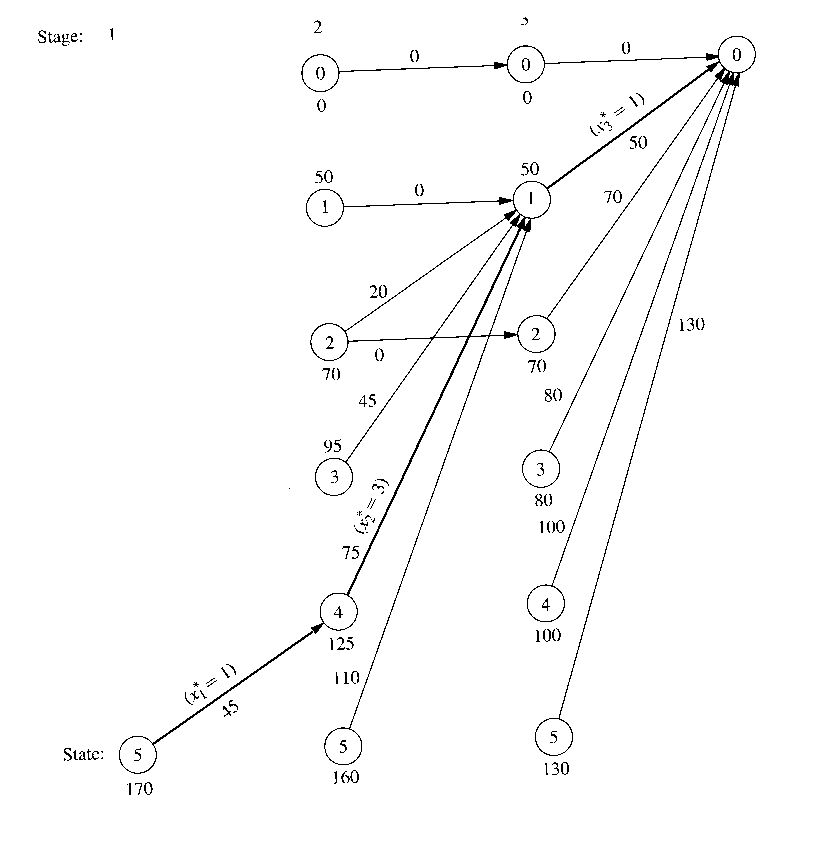
\includegraphics[width=\columnwidth,angle=-2]{figs/teymi4.eps}
\end{center}
\end{lausn}
\end{comment}